\documentclass[final]{article}
\title{Prognosis of prostate adenocarcinoma metastasis using gene activation profiling}
\author{Christopher C Thompson}
%packages
\usepackage[margin=1in]{geometry}
\usepackage{hyperref}
\usepackage{graphicx}
\usepackage{sidecap}
%path definitions
\graphicspath{{Figures/}}


\begin{document}
\maketitle

\section{Definition}

\subsection{Project Overview}

The prostate is a glandular organ of the male reproductive system that helps to
control urinary and reproductive functions.  According to the charity, Prostate
Cancer UK, one in eight British men will  be diagnosed with prostate
adenocarcinoma (henceforth, 'prostate cancer') in their  lifetime \cite{PCUK}.
Men over 50 years of age are often subjected to routine digital examinations,
and/or a urine test (called the Prostate Secreted Antigen, or 'PSA' test) for
signs of prostate cancer.  However the False Positive Rate for these tests remain high \cite{Brawley16} and,
as such,  the gold standard diagnosis is the Gleason test.  In brief, a series
of small needle sized biopsies are taken from the patient's prostate gland.
Each biopsy is processed and scored by a pathologist for signs of abnormal cell
type and structure.  Gleason grades ranging from 2 to 5 are considered not
malignant, whereas scores ranging from 6-10 are considered malignant and provide
an estimation of severity \cite{Humphrey04}.

Contrary to some types of cancer, malignancies that remain local within the
prostate are rarely lethal (survival rate of ~99\%).  However, if a malignancy
born of the prostate undergoes distant metastasis (the process of cancer cell
migration to other sites in the body), the 5-year survival rate drops to ~28\% \cite{CancerOrg}.
Because of this discrepancy, many men opt for radical prostatectomy (surgical
removal of the entire prostate).  While limiting the chance of metastasis,
removal of the prostate results in high morbidity (e.g. inability to control
urination, loss of sexual function, etc).

Unfortunately, there are currently no prognostic tests for prostate cancer metastasis.  The
patient data  that is typically available at the time of diagnosis is not rich
enough to accurately predict the likelihood of prostate cancer metastasis \cite{Brawley16}.   A
model that would be able to predict whether an untreated malignancy is likely to
remain within the prostate or will metastasize to distant sites would be an invaluable tool
in the decision between prostatectomy or surveillance.  To
generate such a model, it is clear that a more distinguishing dataset is required.

One potential solution to this problem is an RNA-seq profile.  In brief, RNA-seq
is a technique that reads and counts RNA sequences in a biological specimen.
What is RNA?  When a gene is activated in a cell, the DNA sequence is read (or
'transcribed') into an RNA molecule.  RNA molecules are then read  into protein
molecules that function in all manner of operations within the cell.  By reading
and quantifying the  RNA molecules that exist in a sample, one may determine
which genes have been activated, and to what degree.  A gene count profile (or 'RNA-seq' profile) is
the estimation of activation for each of the full set of known genes in a biological specimen.

In lay terms, the full set of RNA molecules in a cell can be  thought of as its
blueprint.  And if two set of blueprints were incredibly similar, one would
expect resultant buildings to be similar as well.  In contrast, while a
skyscraper and a lakehouse are both considered buildings, they would likely originate from very
different sets of blueprints.  In the same way, as metastatic cancer cells
behave in drastically  different ways than non-metastatic cells (both metaphorical buildings), one would
assume that their RNA-seq profiles (metaphorical blueprints) would be inherently different.

This difference should be detectable by RNA-seq, though it is unlikely that any
single gene could distinguish metastasis from a local malignancy. The ultimate
goal of this project is to determine the probability of prostate cancer metastasis
from an RNA-seq profile, generated from a prostate biopsy taken during the
Gleason grading procedure.

\subsection{Problem Statement}

The primary questions that this project aims to answer are :
\begin{itemize}
\item Can the risk of prostate cancer metastasis state be predicted from a gene activation (RNA-seq) profile?
\item If so, what genes (individually or in concert) are important for this assessment?
\end{itemize}

The goal of this project is to design a model that predicts the risk of prostate
cancer metastasis using the gene activation profile derived from a patient's
prostate biopsy, taken at the initial Gleason grading diagnosis phase.

To achieve this goal, it is likely that a  significant feature reduction
exercise will be necessary, as each  RNA-seq profile quantifies expression of
20501 human genes.  After feature reduction, a model will be generated to
quantify the risk of prostate cancer metastasis (probability from 0 to 1).
Finally, a function or application will be engineered that receives an RNA-seq
profile as an input and outputs a prediction for future metastasis state.

\subsection{Metrics}

An appropriate metric for the assessment of the probability of a binary class prediction is the
Logarithmic Loss (Log Loss) score.

The equation for log loss is : $$ logloss = -\frac{1}{N} \sum_{i=1}^{N} (y_i
*log(p_i) + (1- y_i) * log(1-p_i)) $$ where \textit{p} represents an observations
predicted probability ($0 < \textit{p} < 1$) and \textit{y} represents the actual binomial class
\{0,1\}.

The log loss function provides a penalty score for each predicted observation in
relation to the difference between the actual class {0,1} and predicted
probability (0:1).  Predictions that are both incorrect and confident are
punished harshly.  For instance, if a model were to return a certain outcome for
binary classification (0 or 1), and that prediction was false (1 or 0), then
infinity would be returned. Thus, in practice, the stastical programs will cap
predictions away from  absolute 0 or 1 prior to log loss assessment.  On the
other hand, an ultra-conservative model that predicted 0.5 for every observation
(effectively not taking either stance in classification) would have a benchmark
log loss score of approximately 0.693147.

\section{Analysis}

\subsection{Data Exploration}

\href{www.http://cancergenome.nih.gov/}{'The Cancer Genome Atlas' (TCGA)} is a
research consortium set up to curate clinical data from thousands of patient
participants, covering an array of cancer types.   The data provided includes basic
clinical information as well as DNA and RNA sequencing of cancer biopsies. These
data sets are updated frequently as new information becomes available.  Thus
each longitudinal download represents a snapshot in an evolving data set.

While detailed genomic and RNA sequence data is control-accessed, pre-processed
gene count data is publicly available.  Data can be downloaded via the
consortium  portal or acquired into data frame format using a package in the R
language.  An R script was written to access the data sets and write them locally
in a python-readable format.  The versions stored in the project repository were current at
the time of the report date.

The clinical data set contains 22 features, of which several are irrelevant
(e.g. all prostate cancer patients are 'male').  Of the features, three were relavant and would be
known at or very near the time of presentation: age, PSA test score, and Gleason
score.  One feature that would also be known but eliminated for ethical reasons is
patient 'race'.  While a higher proportion of Black or Afro-Caribbean men are
diagnosed with prostate cancer, the reasons for this are not fully understood \cite{Shea08} and significant evidence suggests that
race/ethnicity should not be used in cases of genetic / gene activation analysis \cite{Yudel16}.

The outcome variable for this project is contained in the clinical data set,
which is 'pathologyNstage'.  This label is composed of 'n0' or 'n1',
representing local versus metastatic cancer, respectively.  The current
percentage of metastatic cases is approximately 16\%, though this percentage is
likely to increase as the age of the study increases (see Reflection section for
discussion).

\begin{SCfigure}
	\centering
	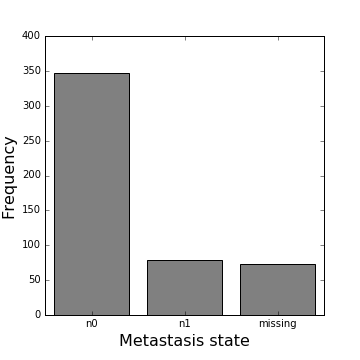
\includegraphics[scale=0.5]{LabelCount}
  \caption{SCFrequency of metastasis state ('pathologyNstage') in the TCGA Prostate adenocarcinoma cohort.\label{MetFreq}}
\end{SCfigure}

When grouped by Gleason score, it is was evident that metastasis rates increased
with cancer severity (Figure 2).  This is  intuitive, yet clearly
not sufficient to determine whether a specific cancer, regardless of Gleason
score, will metastasize or not.  To illustrate, cancers that have been rated at
a Gleason score of '9' are still more likely to belong to the 'n0' class than
the metastasis class.

\begin{SCfigure}
  \centering
  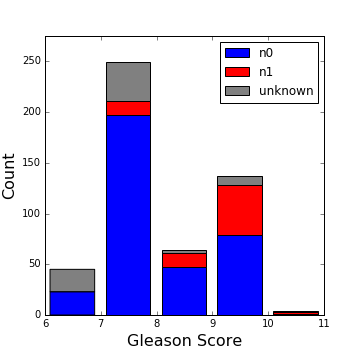
\includegraphics[scale=0.5]{GleasonHist}
  \caption{Frequency of metastasis state grouped by Gleason score.\label{fig:preGSHist}}
\end{SCfigure}

\subsection{Exploratory Visualization}

The clinical information available at the onset of prostate cancer diagnosis is
not rich enough to predict metastasis \cite{Brawley16}.  To corroborate this,
age, PSA score, and Gleason grade were plotted in a scatter matrix in which
each observation is colored based on metastasis state (Figure \ref{fig:ClinSM}).
While Gleason grade seems to correlate weakly to metastasis state, neither age or
(surprisingly) PSA value were proportional to metastasis by visual analysis.

\begin{figure}
  \centering
  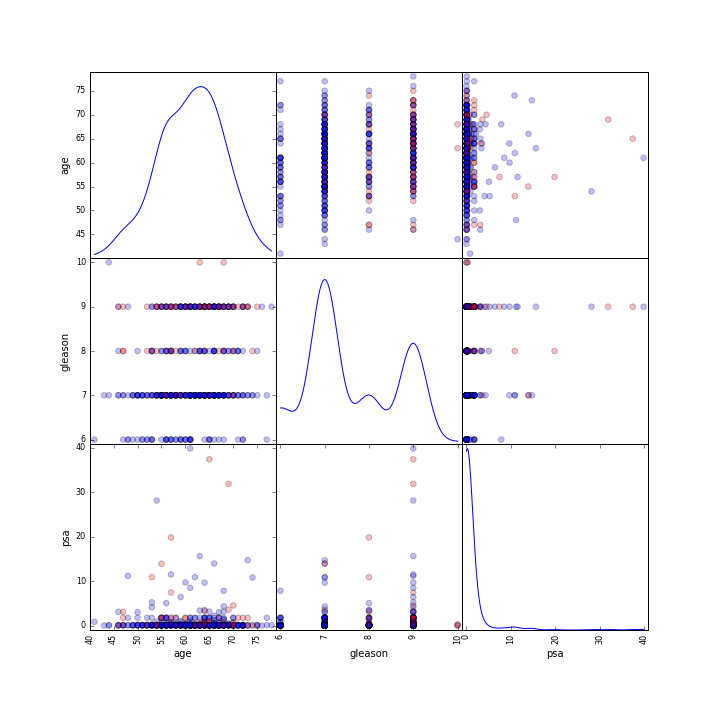
\includegraphics[scale=0.33]{ClinScatterMatrix}
  \caption{Relationship between age, PSA value, and Gleason grade in prostate cancer metastasis class ('n0'- blue, 'n1' - red)\label{fig:ClinSM}}
\end{figure}

The primary data set to be used in this project is the gene count (or RNA-seq)
matrix.  This data set provides a value for gene expression level for every
known human gene. The same patient index links the clinical data set to the
gene count data set, of which 497 are common among the two.  As a pilot
experiment for the project rationale, an F-test was run for every gene feature
in the normalized data set, comparing the 'n0' to 'n1' metastasis states.  The
results from this analysis are  shown in Figure \ref{fig:FDist}, and reveal that
while most genes are not differentially expressed between metastasis states,
some genes do appear to be differentially activated. This indicates that there
are genes that could be used for predictive purposes and validates the project
rationale.

\begin{figure}[h]
  \centering
  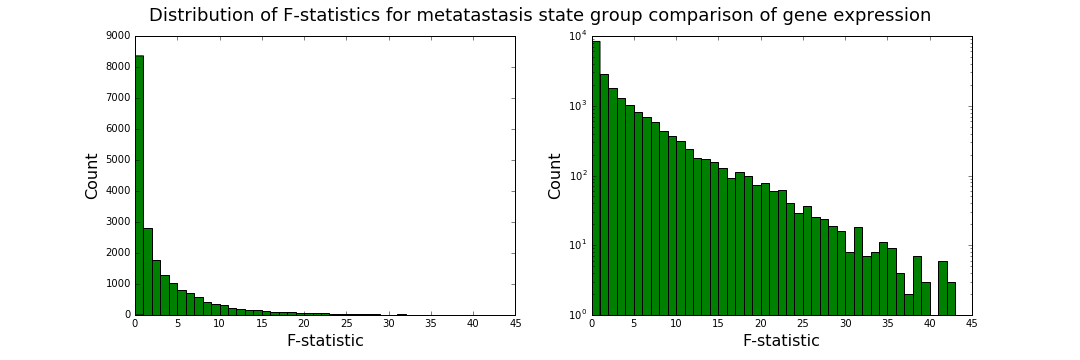
\includegraphics[width = \textwidth]{FDist}
  \caption{Distribution of F-test statistics for the comparison of gene expression levels between the 'n0' and 'n1' metastasis states.\label{fig:FDist}}
\end{figure}

\subsection{Algorithms and Techniques}

The basic outline for project completion is as follows:
\begin{enumerate}
\item Feature selection (filter mechanism)
\item Feature compression into a lower dimensional set
\item Determine which projected features are important for metastasis state discrimination (wrapping mechanism)
\item Subset and train the probabilistic-classification algorithm
\item Measure performance of the trained algorithm on an independent validation ('test') set
\item Compare model performance to the benchmark model performance
\end{enumerate}

The feature reduction exercise will utilize Random Forest Classifier, not as a
classification algorithm, but as a method to measure the ability of each gene to
separate the data set by metastasis class.  Given noisy data, decision trees (and
thus Random Forest) classifiers are prone to overfitting, so parameter limits on
the tree depth and the minimum number of samples that can be split will be defined.
The top portion of genes in 'Gini Importance' will be retained in a subset and carried
into the next project phase.

The reduced feature data set will be compressed further using Principle Component
Analysis (PCA).  PCA is an unsupervised learning technique that transforms a
dataset into its principle components - \textit{i.e.} the orthogonal vectors within the
data that explain the greatest amount of its variance.  By selecting the
the most important components, several features may be combined into a lower
number without significant loss of information.  How many principle components
will be carried into the algorithm training will depend on the amount of variance
each component can explain.  For example, if the first principle component that
explains 95\% of the dataset variance, it would not be necessary to bring any other
principle components forward for further analysis.

The probabilistic-classification algorithm chosen for this task is the logistic
regression ('logit') model.  This algorithm was chosen for its inherent ability
to assess the probability of a binary outcome (\textit{e.g.} metastasis or local
malignancy) based on continuous input variables.  Logistic regression classification is well suited
for noisey data, in that it does not assume that there is any margin or hyperplane that
is capable of separating class labels.  Instead, it returns a likelihood of class assignment
based on the linear combination of input variables as a single term into the logistic
regression equation:

$$ P(class = 1 | X) = \frac{1}{1+e^{-X}}$$

where $X$ originates from :

$$ X = \sum{ \beta_{n}*x_{n}} $$

For algorithm training, a 'solver' is necessary to determine the optimal $\beta$
coefficients to minimize penalties accumulated from a 'cost function'.  There are
several options for both the 'solver' and 'cost function', which also requires
a regularization term, 'C'.

\begin{itemize}
  \item Solver - The 'liblinear' solver is based on a coordinate descent algorithm and
  is ideal for small data sets.
  \item Cost function - the 'l2' cost function is more appropriate in situations
  where features have been pre-filtered or are few in number.  In cases of high
  dimensionality, the 'l1' cost function should be preferred as it practically eliminates
  non-predictive features from contributing to the $X$ term by negating the absolute
  values of the non-predictive features' $\beta$ coefficients.
  \item Regularization term - For situations of high noise (such as this), a larger term
  for $C$ is recommended.  However, the research plan was to optimize this term as needed with
  cross-validation.  Thus it was left at the default value of 1 in the first training instance.
\end{itemize}


\subsection{Benchmark}

As personalized medicine (\textit{e.g.} use of a patient's specific genetic or gene
activation information for therapeutic decisions) has not been established in
mainstream therapy, a benchmark for use of RNA-seq data for prognosis of
metastasis was not available.  Hypothetically, the most conservative model which
predicts every test sample as having 50% chance of metastasis would yield a log
loss score of ~0.69314.

To establish a more fair benchmark for comparison, a logistic regression model
(see methodology below) that incorporated the clinical information that would
normally be known at the time of diagnosis was generated.  These features were
'age', 'PSA score', and 'Gleason score'.

\begin{figure}[h]
  \centering
  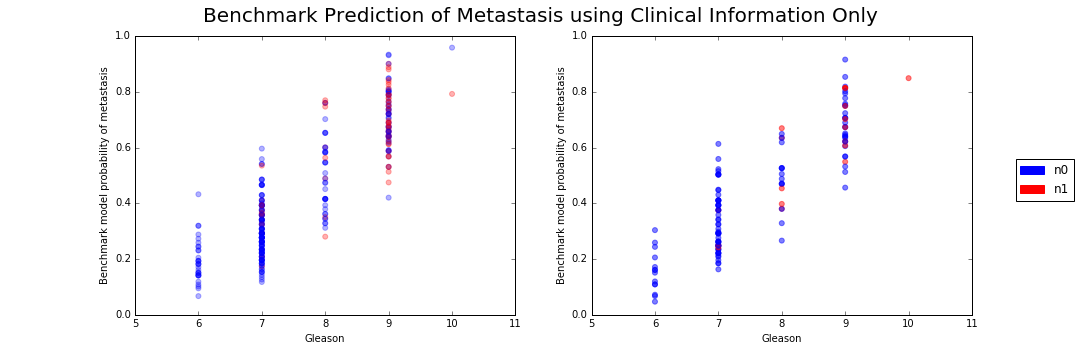
\includegraphics[width=\textwidth]{benchmark}
  \caption{Visualization of a benchmark logistic regression predictive model performance.\label{fig:benchScat}}
\end{figure}

\begin{table}
  \centering
  \caption{\label{tab:benchcoefs} Benchmark logistic regression model coefficients for clinical features}
    \begin{tabular}{l l}
      \hline
      Feature & Coeffiecent \\  \hline
      age & -0.067344 \\
      PSA Value & 0.025574 \\
      Gleason Grade & 0.858936 \\
      \hline
    \end{tabular}
  \end{table}

The coefficients for the three features in the model (representative values shown in Table \ref{tab:benchcoefs}) exhibited that
Gleason score was by far the most predictive (approximately 0.85), and that age and
interestingly PSA score (which is the current default test that doctors rely on
for prostate cancer risk)  provided very little use in classification.  Figure 5
(left) shows the relationship between Gleason score and the benchmark model's
prediction of metastasis.  Figure 5 (right) shows the distribution of metastasis
probabilities, grouped by actual metastasis state.

The log loss score from this benchmark analysis ranged from approximately 0.59 - 0.62 across 5 different runs (See Table \ref{tab:performance}), and
thus could be considered marginally more useful than a '50\% model'.

\section{Methodology}

\subsection{Source Files}

The datasets were retrieved from the TCGA portal using an R package,
\href{https://cran.r-project.org/web/packages/TCGA2STAT/index.html}{TCGA2STAT},
and written to the local drive in \href{https://github.com/wesm/feather}{feather} format,
which is python-readable.  The R script used and feather files are
available in this project's GitHub repository
\href{https://github.com/CCThompson82/MLE\_capstone}{MLE\_capstone}.  All
algorithms were imported from the
\href{http://scikit-learn.org/stable/}{scikit-learn} library, version 0.17.

\subsection{Data Preprocessing}

Samples with a Gleason score of 6 were homogenous in metastasis state (all
'n0'), though many cases were not labeled.  In order to make more efficient use
of the  TCGA RNA-seq data set, 'n0' was imputed for all samples where no label
existed and  Gleason grade was defined as 6.  The reasoning behind this decision
was that those with low grade  malignancy are usually not screened from
metastasis and thus the lack of data label  probably reflected the
dispensibility of the metastasis test in cases of mild malignancy. From a
machine learning perspective, this step allowed more efficient use of a rather
small dataset.  Given a much bigger data set, then this assumption would not be
necessary, and  all cases with missing label could be excluded.  Indeed, for
cases scored 7-10 on the Gleason scale where no labels were included in the
clinical data were excluded from further analysis.

\begin{SCfigure}
  \centering
  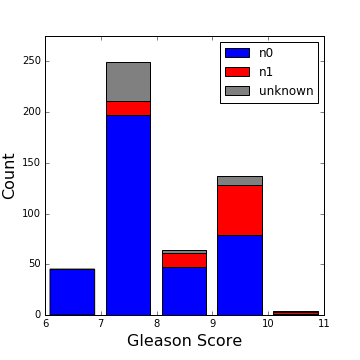
\includegraphics[scale=0.5]{GleasonHist2}
  \caption{Distribution of known clinical features grouped by metastasis state (blue: 'n0', red: 'n1').\label{fig:postGSHist}}
\end{SCfigure}

The gene count data retrieved from the TCGA portal was in an intermediary
format.  While the raw RNA-sequence reads had been processed into gene
activation estimations, each specimens profile required normalization for
cross-sample comparison.   Therefore, the initial gene count dataset was transformed to
transcripts per million (TPM) format.  This dataframe ('X') was the base upon
which further feature reduction and test train splitting would be performed.

\subsection{Implementation}

Feature reduction was completed in two steps.  The first was to utilize the
generation of a
\href{http://scikit-learn.org/stable/modules/generated/sklearn.ensemble.RandomForestClassifier.html#sklearn.ensemble.RandomForestClassifier}{Random
Forest Classifier} to supply information regarding the importance of each gene
in the separation of metastasis states.  As the Random Forest model was not
intended for actual classification purposes (not optimal due to the small sample
size of the dataset), only key default parameters were altered. Specifically,
the maximum tree depth was limited to 3 nodes, and the minimum number of samples
that could be split was limited to 30.  These parameter choices were intended to
limit variance.  The 'Gini Importance' of each feature was retrieved from the
model and the genes ranked in the order of importance.

From this list, the original plan was to retain the top \textit{k-}number of
genes for PCA compression.  However, run to run observation revealed that the
set of genes  was rarely identical.  Many genes, such as \textit{gne} were
present in every case, however their ranking changed each run, which affected
the subset retained in each run.  To address the issue of feature stability, the Gini
Importance selection process was repeated across 5 different random seeds, with only
the genes present in the top \textit{k} of every epoch kept.  In this
solution, \textit{k} was set to 100 and resulted in a relatively stable selection of
~11-18 genes.  This subset was scaled to standard mean and unit variance using the sklearn
\href{http://scikit-learn.org/stable/modules/generated/sklearn.preprocessing.StandardScaler.html#sklearn.preprocessing.StandardScaler}{Standard Scaler} in preparation for further compression.

The second phase of Feature reduction was \href{http://scikit-learn.org/stable/modules/generated/sklearn.decomposition.PCA.html#sklearn.decomposition.PCA}{Principle Component Analysis}
compression. The PCA algorith ranks a data set's orthogonal vectors by variance, and transforms the data set to comply with the identified eigenvectors.  The percent explained
variance can be determined from associated eigenvalues in this process.  Moreover, the contribution
from each gene of the the \textit{k-}gene subset can be determined and is shown for the first
3 PCs in Figure \ref{fig:pcaEV}.

\begin{figure}[h]
  \centering
  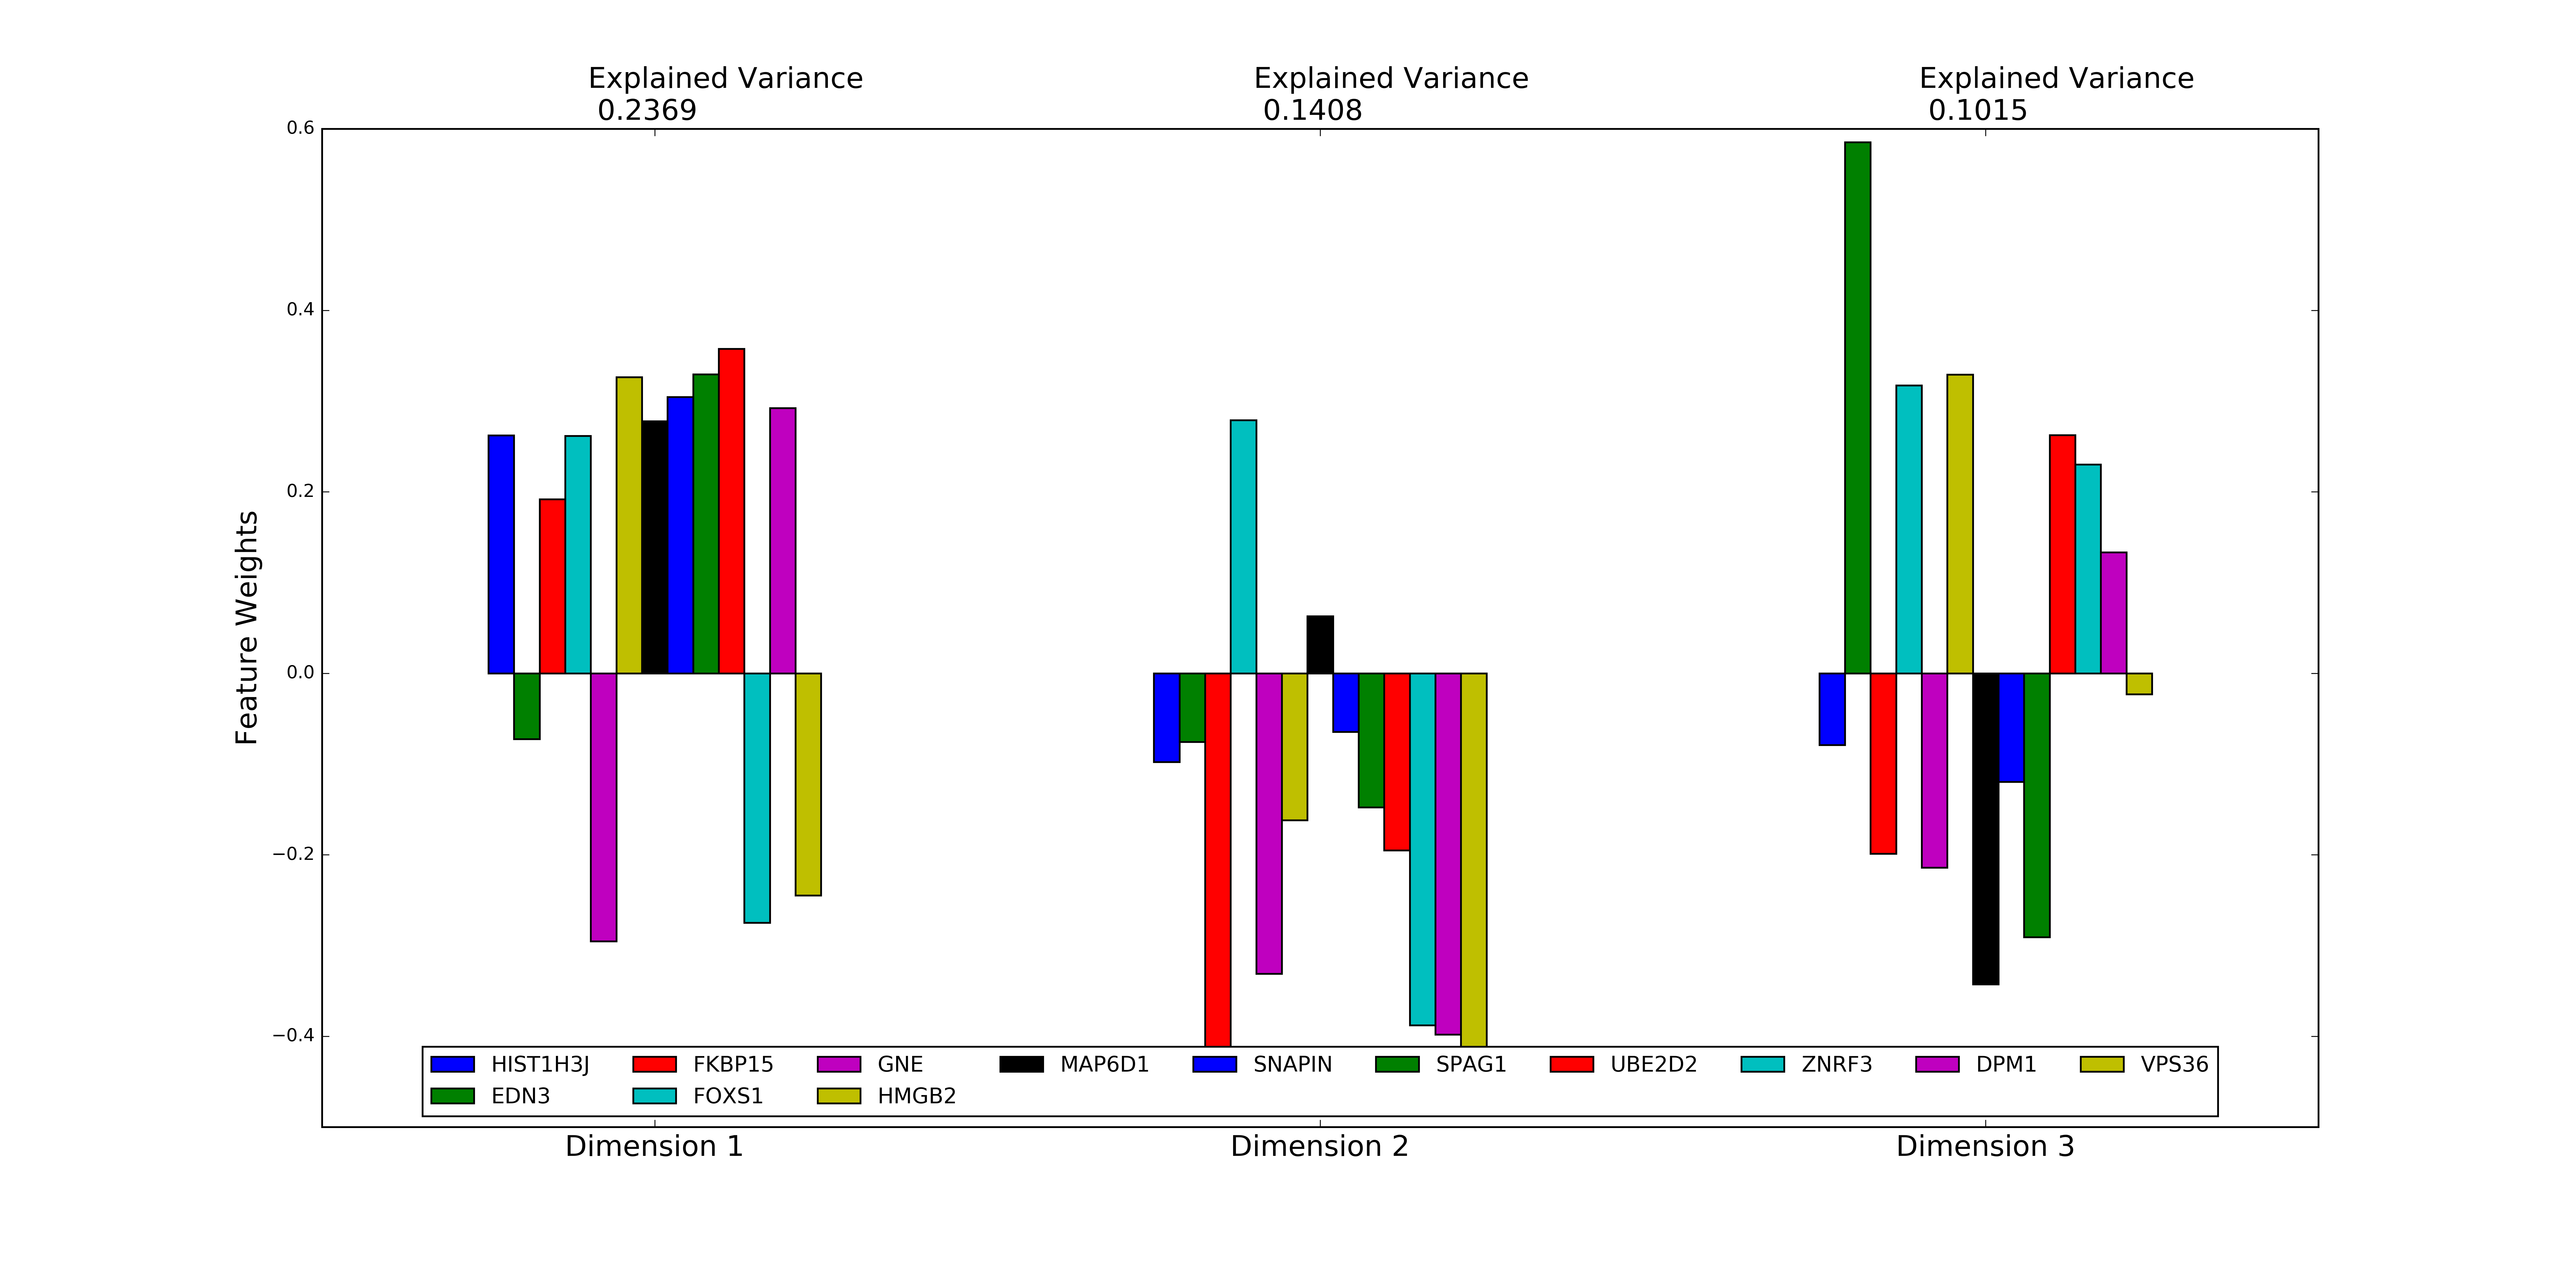
\includegraphics[width=\textwidth]{pcaEV}
  \caption{Explained variance and gene feature contribution to the first three principle components of the PCA transformation.\label{fig:pcaEV}}
\end{figure}

This 3-feature dataset was then partitioned using the same indices from the
first \href{http://scikit-learn.org/stable/modules/generated/sklearn.cross_validation.train_test_split.html}{Train Test Split}
performed prior to the benchmark model generation.  In detail, this
split partitioned 70\% of the samples into the training set, with 30\% being held
out for validation.  The data was stratified by Gleason score, which was used
as a surrogate measure for cancer severity. While not a perfect solution, this
decision was made to ensure that 'easy' (\textit{e.g.} mild or extremely severe
malignancies) and 'difficult' (\textit{e.g.} malignancies on the border between
moderate and severe) cases would be distributed equally.  Another option would
have been to stratify by  metastasis label (see 'Reflection' section for  %set up reference label pair here
discussion on this decision).

The training data set was then fed into a
\href{http://scikit-learn.org/stable/modules/generated/sklearn.linear_model.LogisticRegression.html}{Logistic
Regression Classifer} model.  For this learning, the class-weight parameter was
set to 'balanced' in order to guard against confounding effects of the
unbalanced label set in model performance.  The regularization ('C') parameter
was left at the default value of 1.  The C term is inversely proportional to the
penalties awarded for misclassified samples. Hypothetically, a higher
regularization term may have increased performance, however this was to be
determined empirically in future optimizations.

Results were visualized using graphs generated with the
\href{http://matplotlib.org/index.html}{matplotlib} package.  Performance of the
logistic regression model was tested against the held-out test set using the
\href{http://scikit-learn.org/stable/modules/generated/sklearn.metrics.log_loss.html#sklearn.metrics.log_loss}{log
loss} metric.  For references, the
\href{http://scikit-learn.org/stable/modules/generated/sklearn.metrics.fbeta_score.html}{F$\beta$
score ($\beta$ := 2)} and
\href{http://scikit-learn.org/stable/modules/generated/sklearn.metrics.matthews_corrcoef.html}{Matthews
Correlation Coefficient} scores are also listed, though they describe the
performance of the algorithm to correctly classify metastasis state and do not
measure performance in probabalistic prediction.  Both the graphical analysis
and metric reports were generated for each testing cycle using the scripts
supplied in the
\href{https://github.com/CCThompson82/MLE_capstone/tree/master/Support%20Files}{'Support
Files'} folder in the GitHub repository.

\subsection{Refinement}

In order to optimize the C parameter, a \href{http://scikit-learn.org/stable/modules/generated/sklearn.linear_model.LogisticRegressionCV.html#sklearn.linear_model.LogisticRegressionCV}{Logistic Regression CV}
classifier generated using 4 fold cross-validation across a 10-log range for C.
Performance was measured using \href{http://scikit-learn.org/stable/modules/generated/sklearn.metrics.log_loss.html#sklearn.metrics.log_loss}{log loss}
as the  scoring function.  This process yielded a maximum term for C, 10000.

\begin{figure}
  \centering
    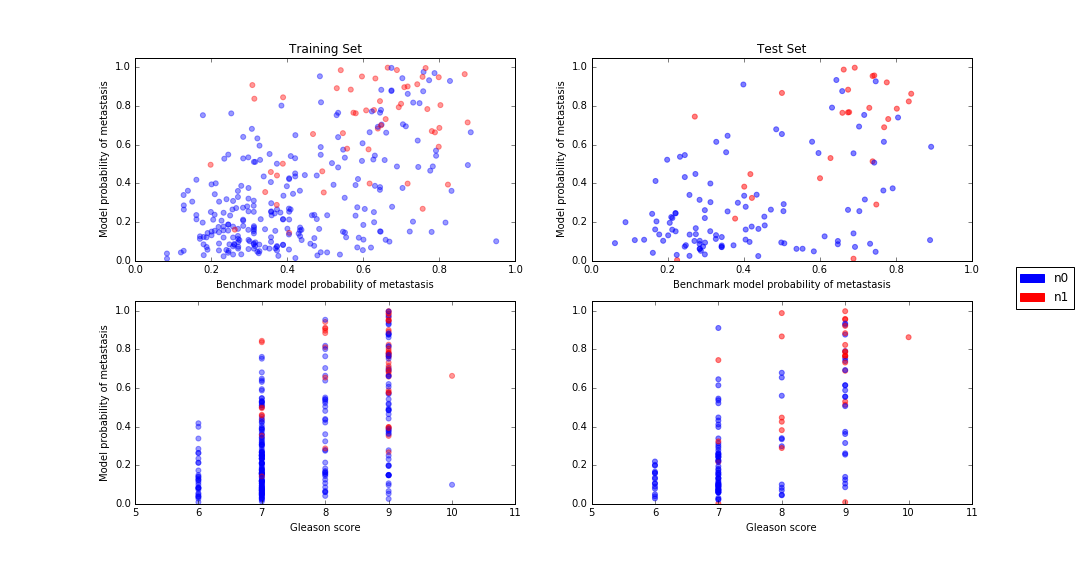
\includegraphics[width=\textwidth]{optPC3}
    \caption{\label{fig:PC3}Optimization of the regularization parameter acheives minimal improvement on model performance.}
\end{figure}

Because Gleason grade was clearly the most important clinical feature in predicting
prostate cancer metastasis, it was added back to the training feature set to see
if any improvement in performance could be acheived.

\begin{figure}
  \centering
  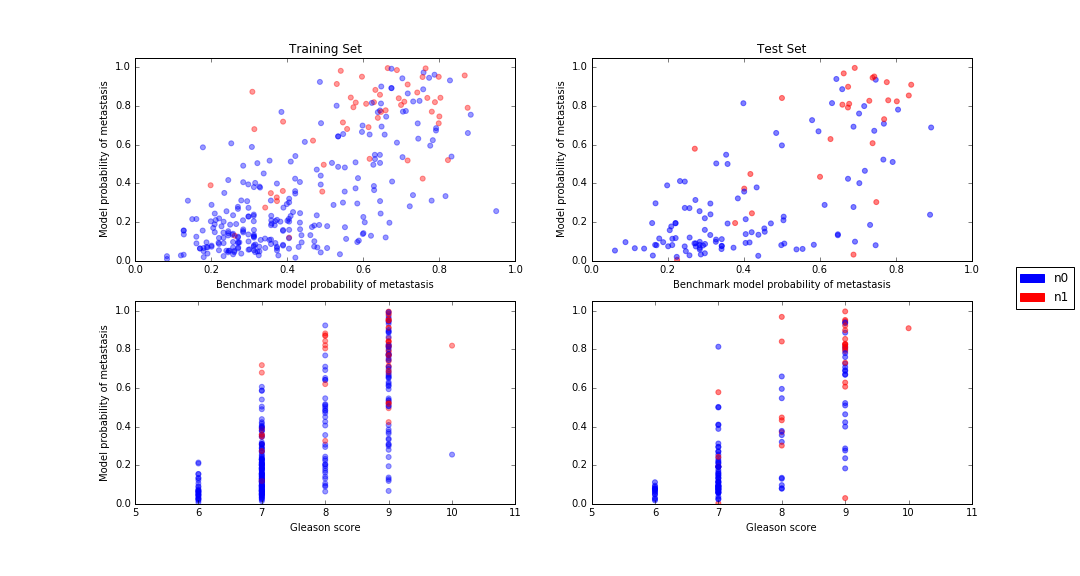
\includegraphics[width=\textwidth]{PC3Gleason}
  \caption{\label{fig:PC3GG}Addition of Gleason grade to the PC model acheives minimal improvement on model performance.}
\end{figure}

\section{Results}

\subsection{Model Evaluation and Validation}

\subsubsection{Final Model}

The final logistic regression model receives 2 feature variables:

\begin{enumerate}
\item Gleason score
\item the first 3 PCs from a \textit{k-}gene subset of expression values
\end{enumerate}

\begin{table}
  \centering
  \caption{\label{tab:FFcoefs}}
    \begin{tabular}{l l}
      \hline
      Feature & Coefficient \\ \hline
      Gleason Grade & 0.523239  \\
      First PC & 0.603294 \\
      Second PC & -0.372170  \\
      Third PC &  -0.190558 \\
      \hline
    \end{tabular}
\end{table}

The coefficients for Gleason grade and the first PC were routinely equivalent,
indicating they contribute roughly evenly to dependent variable prediction.  The
2nd and 3rd PCs do not contribute as much to the logistic regression decision
function (see Table \ref{tab:FFcoefs}).  The optimal regularization parameter
was regularly determined as the maximum value tested, which is an indication of
noisy (\textit{i.e.} not linearly separable) data set.

\begin{figure}[h]
  \centering
  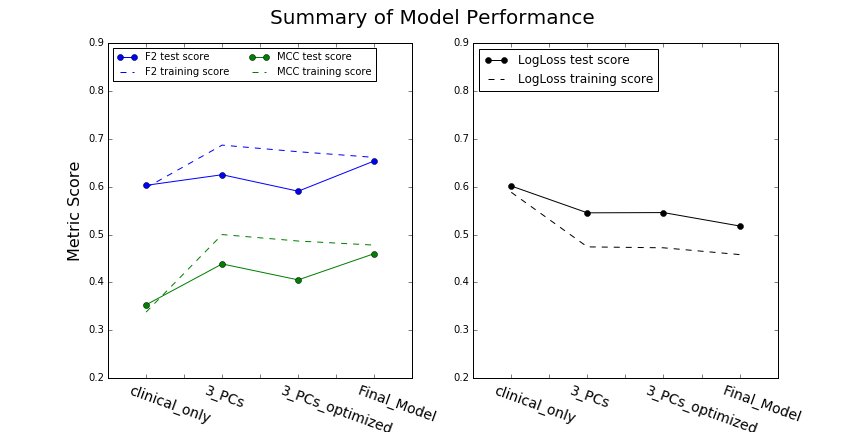
\includegraphics[width=\textwidth]{FF}
  \caption{Summary of the change in metric score over the optimization course of the project.  The final model, that incorporates a single principle component with Gleason score performs better than the benchmark model in three metrics tested.\label{fig:FM}}
\end{figure}

The error / accuracy rate of three performance metrics was often similar
between the training sample and test sample set predictions, indicating the
model was not over-fit.  As only 2 feature  variables were incorporated into the
training of the final model, the possibility of bias was present.  However

\subsubsection{Test set Validation}

\begin{table}[h]
\centering
\caption{Performance across 5 random seeds\label{tab:performance}}
\begin{tabular}[h]{ r c c c }
\hline
Seed & Final Model LogLoss & Benchmark LogLoss & Improvement over Benchmark (\%) \\  \hline
1 & 0.496309 & 0.605505 & 18.0 \\
12 & 0.479994 & 0.618392 & 22.4 \\
123 & 0.556008 & 0.621997 & 10.6 \\
1234 & 0.51460 & 0.615772 & 16.4 \\
12345 & 0.467942 & 0.595507 & 21.4 \\
\hline
\end{tabular}
\end{table}

This project's strategy was to leave out 30\% of the original dataset to use as a
true validation of the models' generalization capability.  The final model validation
set log loss score ranged from 0.467 to 0.56 across five different random state
seeds.  Each value in this range was lower than the minimum benchmark score in the
same 5 runs.  Analyzed on a run by run basis (in which the training and test set cases
are consistent), the final model acheived between 10.6 and 22.4\% improvement over
the benchmark.

\subsection{Justification}

The final logistic regression model performed better in predicting the
probability of prostate cancer  metastasis than the benchmark model in every
run.  Over the five consecutive runs described above, an average improvement of
approximately 17\%  over the benchmark.

In order to test sensitivity of the model, a pipeline function was implemented
that received RNA-seq profile and returned the final model probability of
metastasis.  To test the functionality of the pipeline application, all RNA-seq
profiles where the label was missing and Gleason grade was 7-10 were subjected
to prediciton.  Results from this analysis are shown in Figure
\ref{fig:missing}.  Clearly several of these cases were risk for metastasis
according to the model and risk appeared to be correlated  to Gleason grade (not
surprising as Gleason grade is a positively correlated to metastasis
probability, Table \ref{tab:FFcoefs}).

\begin{figure}[h]
  \centering
  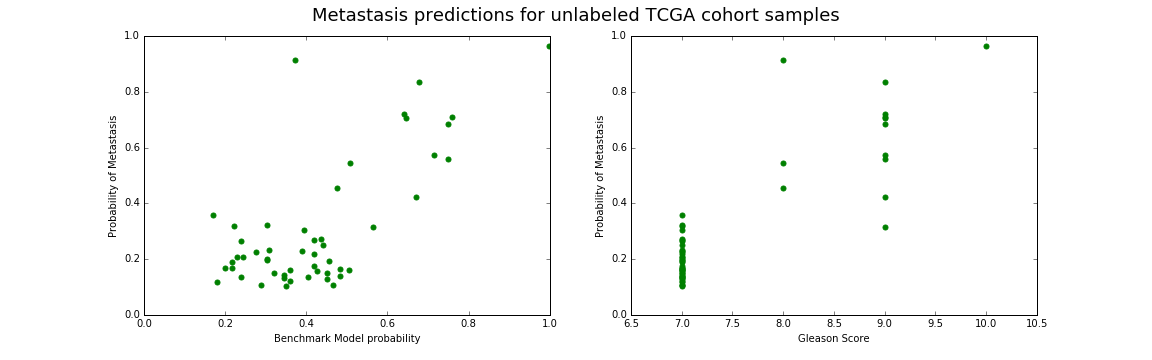
\includegraphics[width=\textwidth]{missing}
  \caption{\label{fig:missing}Metastasis predictions for unlabeled TCGA cohort samples.  TCGA cohort patient samples that did not include a metastasis label and were Gleason range 7-10 were omitted from model learning and validation.  Samples are subjected to the risk analysis function and plotted against the benchmark model prediction (left) and Gleason score (right).}
\end{figure}

As a true test of senstivity, matched patient benign controls were run through the
pipeline function.  These samples originated from areas of the prostate where
no malignancy was evident (though malignancy was present within the same prostate
gland in each case).  As expected, the density of metastasis probability was was
right-skewed with the vast majority of predictions falling in the <0.20 range.

\begin{SCfigure}
  \centering
  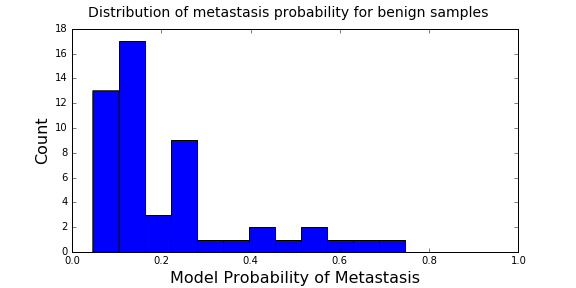
\includegraphics[scale = 0.5]{Sensitivity}
  \caption{\label{fig:Sensitivity} Analysis of risk from matched, benign controls from the TCGA cohort data reveal that the final model is stringent.  Samples from this cohort were taken from benign areas of patient prostates where malignancies were present.  The majority of samples are predicted with a low probability of metastasis.}
\end{SCfigure}

\section{Conclusion}

\subsection{Free-Form Visualization}




\subsection{Reflection}

\subsubsection{Objective}

The purpose of this project was to generate a model capable of supplying a
patient and doctor with a metric for risk of prostate cancer metastasis that was
more useful than simple use of the 'Gleason Score'.  To accomplish this, RNA-seq
(gene activation profile) was explored as a potential inroad into personalized
therapy for newly diagnosed prostate cancer patients.  There were several issues
that made this task difficult:

\begin{enumerate}
\item Small, wide sample data - the effective
dataset (containing Gene Activation profile and a metastasis label) was 446
samples by 20501 gene features.
\item 'Inaccurate' / 'Pre-mature' data labelling -
The TCGA cohort is regularly updated and those listed as non-metastatic at the
time of update could become metastatic at a later date.  Indeed many of the 'non-metastatic'
observations are still predicted to have a high chance of metastasis, despite many of the cases being used for
training of the model algorithm (See Figure \ref{fig:n0}
\item Noise in the data -
no single gene or biomarker had been reported as capable of efficiently
separating non-metastatic and metastatic cancers(corroborated in this project,
Figure \ref{fig:separate}).
\end{enumerate}

\begin{SCfigure}
  \centering
  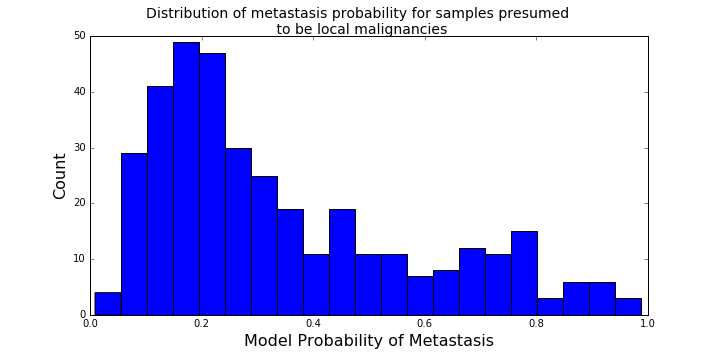
\includegraphics[scale=0.5]{N0Analysis}
  \caption{\label{fig:n0} Metastasis prediction of samples labeled as non-metastastic}
\end{SCfigure}

Thus from a machine learning perspective, it was clear from the project's onset
that feature reduction and appropriate model selection would be paramount to
success.

\subsubsection{Feature Selection}

There are many techniques for feature reduction.  One avenue explored was
feature elimination via a wrapping mechanism.  However this approach was very
slow and provided inconsistent results in which features and how many features,
were important. A different approach was to utilize the
training of an ensemble Random Forest classifier, not for its use in
classification, but in order to access its assessment of which genes were most
informative in separation of the metastasis classes.  An iterative process was
utilized to stabilize the gene set upon which PCA transformation would be performed. Implementation of this feature was not essential for increased final model
validation performance, thought it did reduce the run to run variation in predictive
performance.

Importantly, visualized individually, none of this reduced k-gene set could separate the metastasis
state linearly.

\begin{figure}[h]
  \centering
  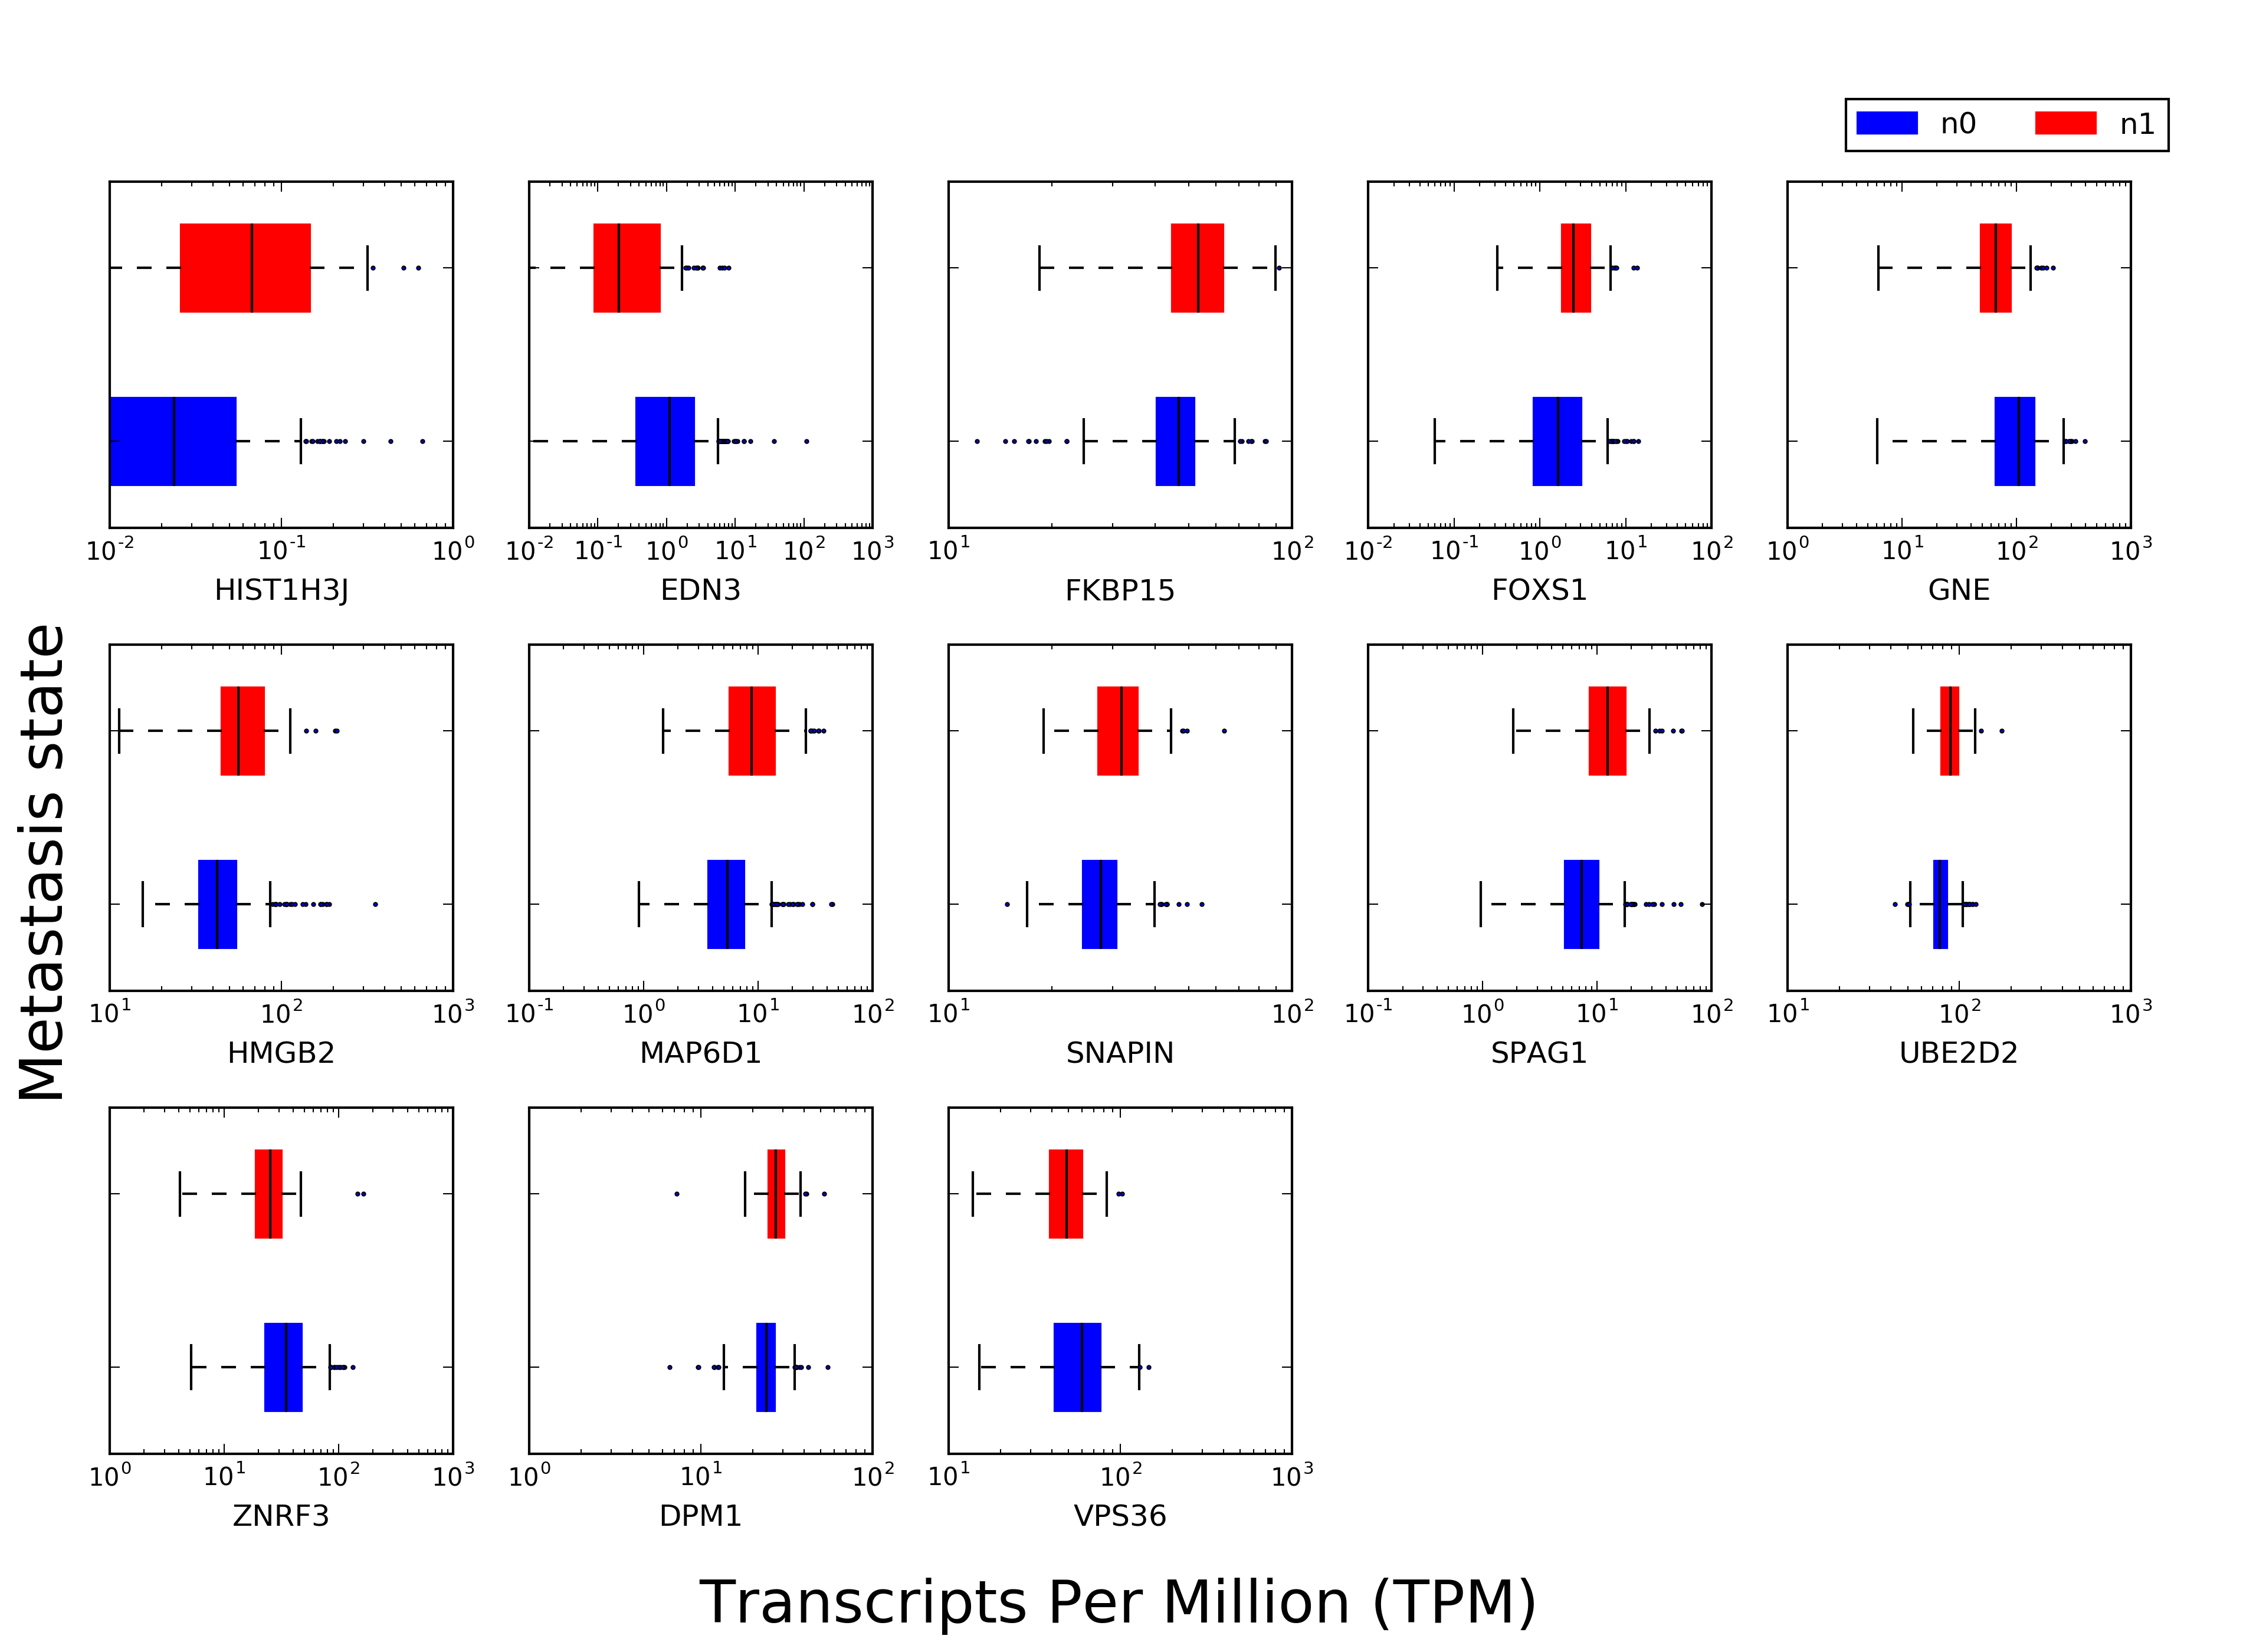
\includegraphics[width=\textwidth]{boxplots}
  \caption{\label{fig:separate}Genes with the highest 'Gini Importance' scores were still not able to distinguish metastasis class.}
\end{figure}

The initial plan at this point was to provide the full complement of principle components to the logistic regression classifier as training data, and
subsequently use each component's coefficient to  assess which were most able to
explain the independent variable in a \href{http://scikit-learn.org/0.15/modules/generated/sklearn.feature_selection.RFECV.html#sklearn.feature_selection.RFECV}{Recursive Feature Elimination}
wrapping function.  However, graphical analysis of the principle component scatter matrix, grouped by
metastasis state (Figure \ref{fig:pcaScatter} ) curiously showed that the first principle
component seemed to generate distinct gaussian distributions for each of the metastasis states, despite the fact that PCA is an unsupervised technique.  This result was consistent independent of
whether 5 through 500 genes were 'Gini' selected for PCA transformation.

How could this be?  This result would be expected if a transformation technique
such as linear discriminant analysis (LDA) had been employed, as LDA uses data
label in order to determine the component vectors where class label is
discriminated the most.  PCA, on the other hand, is an unsupervised technique
and had generated what appeared to be a discriminant component in the absence of
label information.  However, upon reflection, it is perhaps not surprising that
the eigenvector where the most variance in the data subset was contained (\textit{i.e.}
the first principle component) would separate the class labels, given that
\textit{only genes where a 'significant' difference in gene expression between the
class labels} were retained and provided to the PCA model.

By creating a pipeline from the  Gini Importance filter directly into the PCA
transformation, something similar to
\href{http://scikit-learn.org/0.16/modules/generated/sklearn.lda.LDA.html}{Linear
Discriminant Analysis} had been generated.  Indeed, exploration of an supervised
LDA compression of the 20-feature set yielded a similar level of performance in
the final model compared to compression via Gini Importance to PCA pipeline.

\begin{SCfigure}
  \centering
  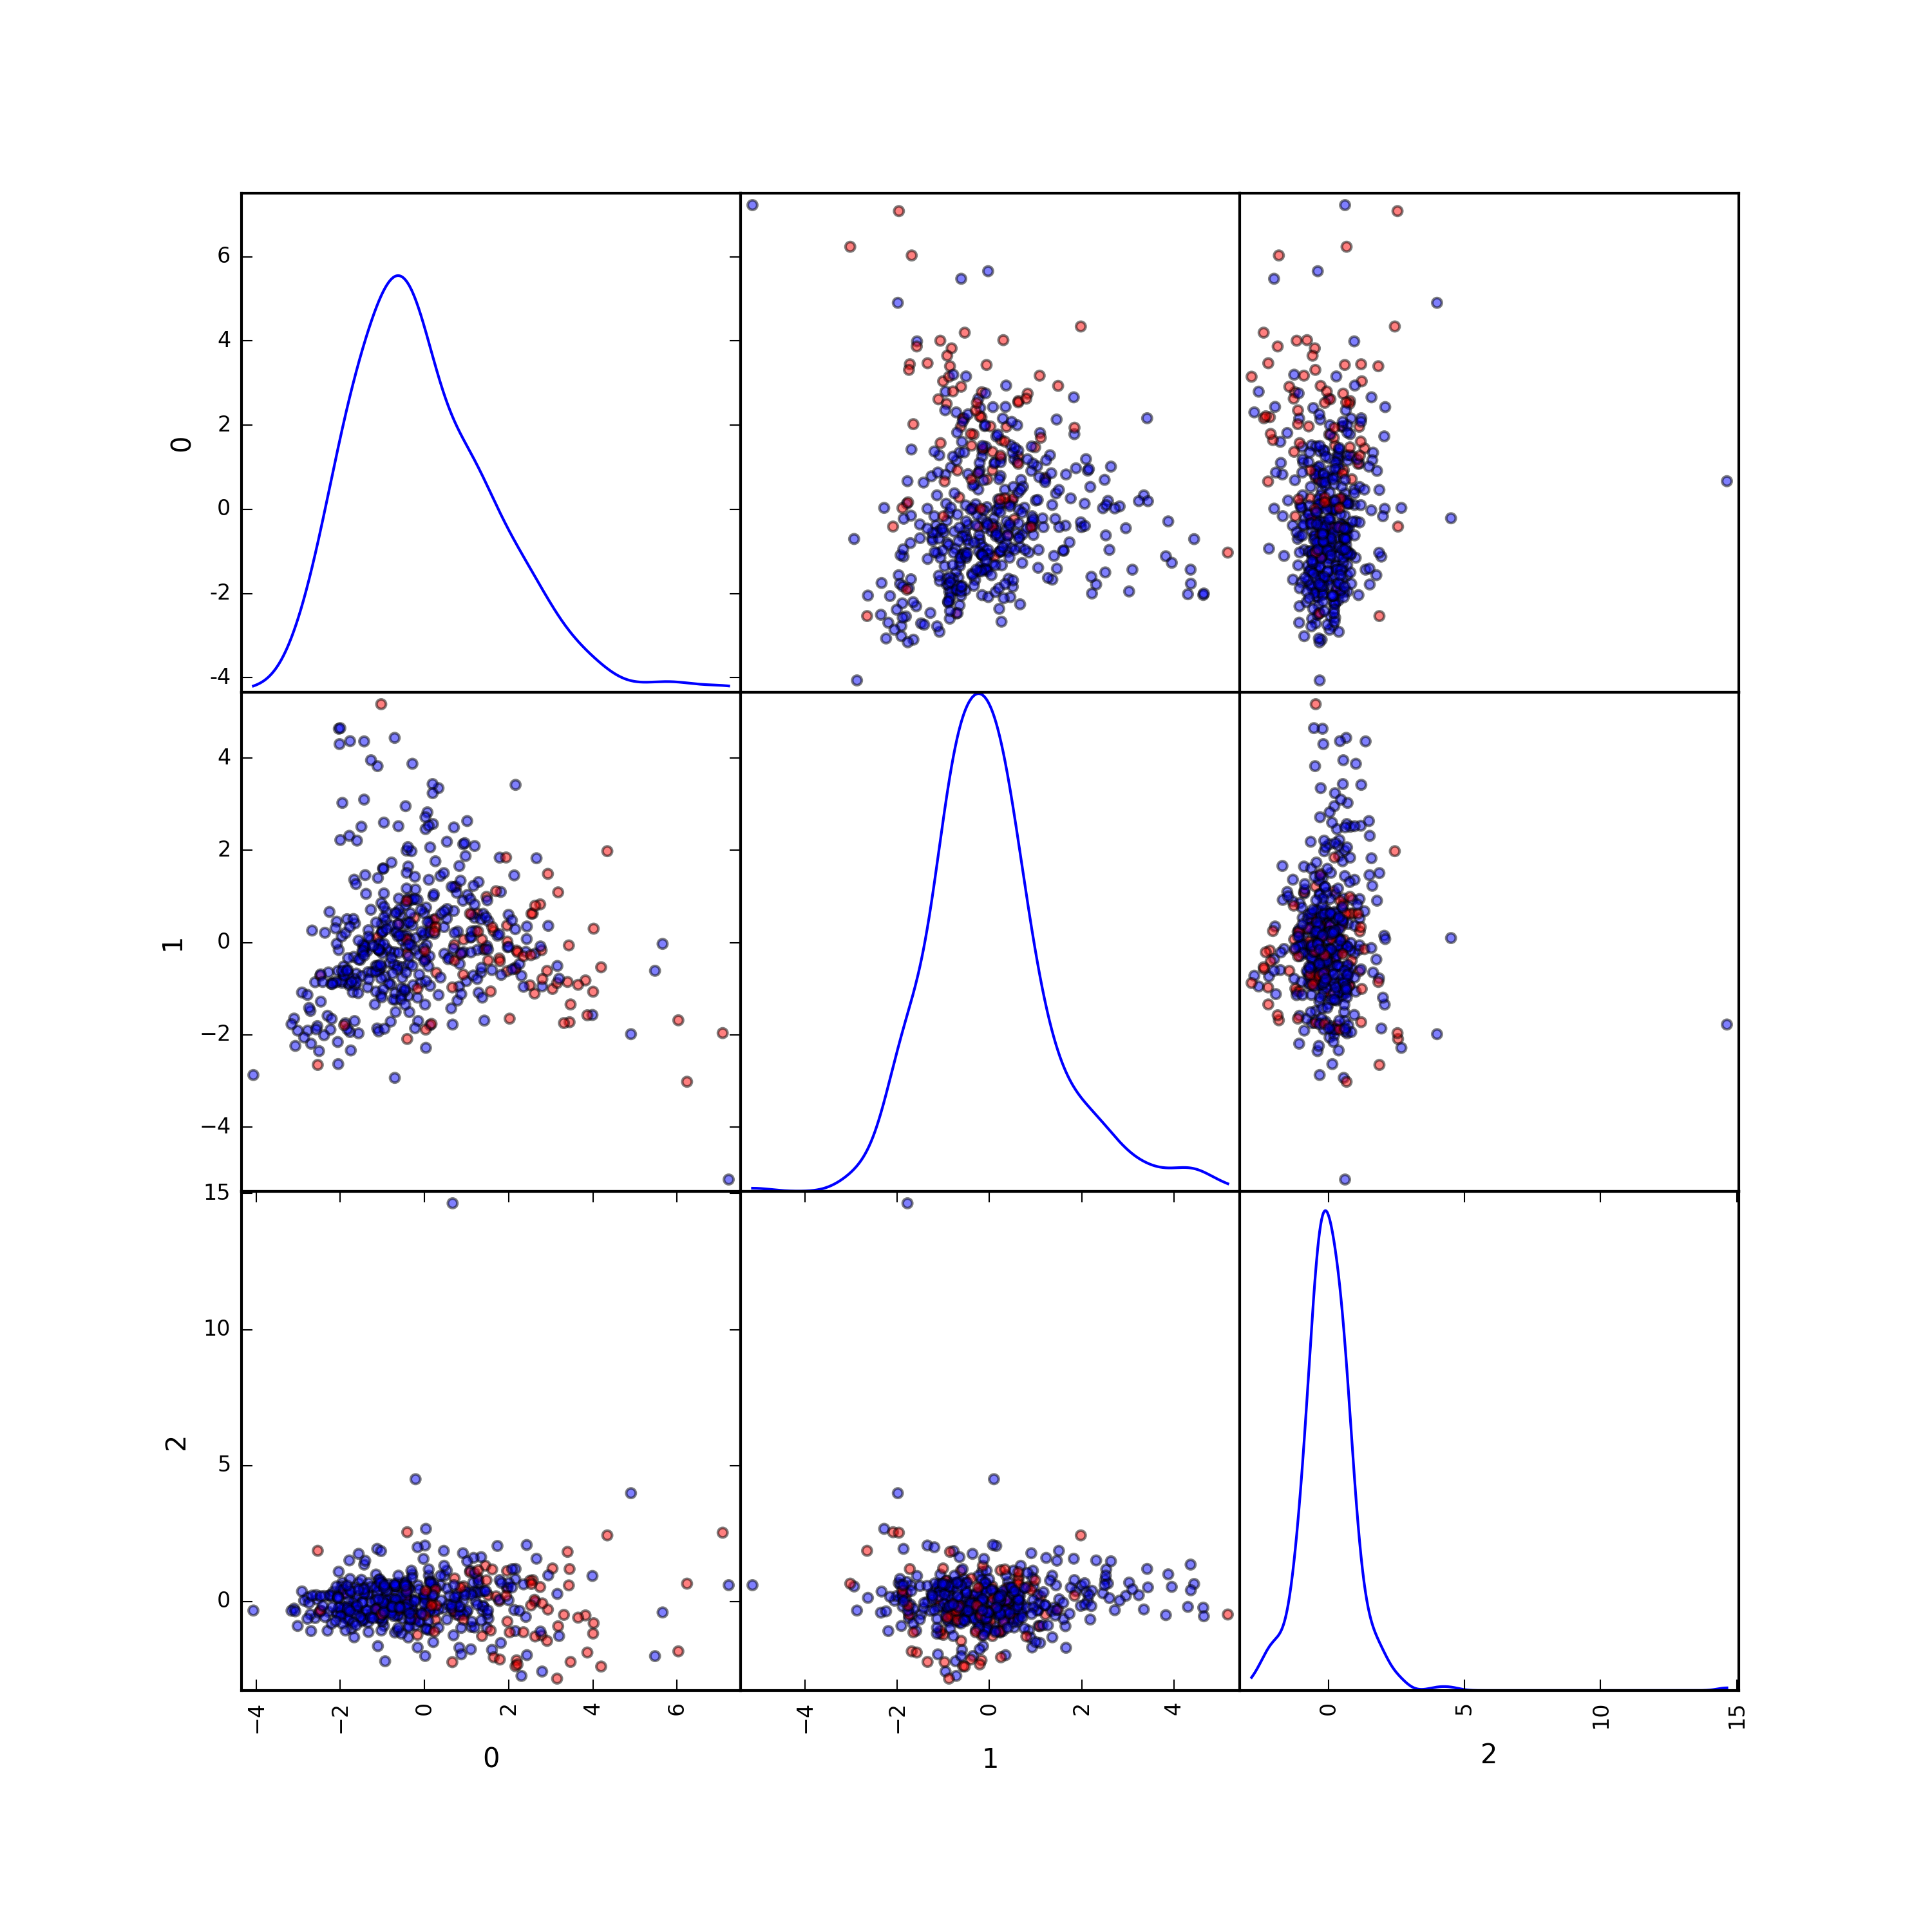
\includegraphics[scale = 0.5]{pcaScatter}
  \caption{\label{fig:pcaScatter}Analysis of PCA transformation of a k-gene feature subset.  The first principle component of PCA transformation separates metastasis state more efficiently than any single gene from the input set.  The second and third principle components are also shown for reference.}
\end{SCfigure}

The 3-component feature set taken from this transformation was split on the same indices that were generated in
the training and validation sets used in the benchmark analysis.  This was done
to aid in model to model comparisons within each run.  To note, this split was
originally stratified on the y-label (metastasis state).  However, after
observing moderately inconsistent results for final model validation
performance, the decision was made to stratify by Gleason score (Cancer
severity) of the samples.   This decision ensured that difficult cases - those
in the middle range of severity - were equivalently distributed among the
training and test sets, vastly reducing the run to run variation.

\subsubsection{Model Selection}

Having completed a feature selection and compression technique, in which at
least the first principle component seemed capable of distinguishing among
metastasis class via graphical analysis (**Figure 11**), a logistic regression
classifier was chosen as the predictive model.  Logistic regression was
preferred  to other hyperplane-based techniques, such as support vector
machines (SVM) due to the noise that was expected in the compressed dataset.
SVM classifiers attempt to define the hyperplane by which the margin between
the class labels is maximized.  In situations where data is not easily
separable, this result can be unstable, and  at times, arbitrary.  Moreover,
SVM does not provide a true probability of class assignment, as was the
objective of the project.  In contrast, logistic regression assumes that no
feature  is capable of explaining the outcome variable, but that the
combination of features  should be able to provide a probability of class
assignment.  This assumption holds true for the RNA-seq dataset employed in
this project.  Moreover, as the objective of this project was to provide a
probability of metastasis, the output of logistic regression classifier is
perfectly suited.

\subsubsection{Training and Optimization}

Separate Train and Test indices were stratified based on cancer severity prior
to the benchmark analysis and the final PCA compressed (3-components) were
subset into these indices.  Logistic regression classifier was trained and
optimized on the Train set, prior to validation on the Test set.  Gleason score
was added as a feature to this model and the 2nd and 3rd principle components
were eliminated from the model after determining that they did not contribute to
model performance.

The final release version of the code was run across 5 seeds and performance in
the primary metric (log loss), and secondary metrics (F2 and MCC) were recorded,
compared to the benchmark.

\subsubsection{Model Performance}

In every run tested, the performance of the final model exceeded performance of
the benchmark model by at least 14\% in log loss score.  The pipeline exhibited
in this project could be re-appropriated for other types of RNA-seq based
classifications.  By looking for individual genes whose activation level explain
a certain condition, researchers may be missing the opportunity to provide
valuable disease prognosis.  Instead, by performing a feature selection and
compression, researchers may be able to predict disease more regularly at the
sacrifice of knowing \textit{exactly} what genes are causal.

Importantly, I hypothesize that as the TCGA cohort study is updated
longitudinally, its performance will be more accurate.  This is due to the
nature  of analyzing an on-going cohort trial.  In the context of a machine
learning problem,  sample labels will only move in one direction (from
'non-metastatic' to 'metastatic', never \textit{vis-a-versa}).  Therefore those patient
samples predicted with a high  probability of metastasis, currently labeled as
non-metastatic, would be correctly classified in future validation.

Unfortunately in the context of the TCGA cohort study, the link between patient
and barcode has been broken for ethical reasons, meaning that such patients with
high risk  can not be identified for extra care in monitoring metastasis.


\subsection{Improvement}

There is still bias in this model due to the small sample size.  Increased
number of specimens could allow more resolution / stability in feature selection
and  compression.  For each iteration of the code, a handful of genes selected
from the 'Random Forest filter' is altered, though 10-15 remain identical.

Evidence here and elsewhere suggests that no gene or principle component could
be capable of separating  metastasis state classes, and thus logistic regression
is an excellent long term  model for prediction.  However, it is possible that
other sources of information  could help improve model accuracy, including
genetic or epigenetic specimen data.  Ultimately only increasing the sample size
will be able to significantly increase the resolution for prostate cancer cancer metastasis
prediction.

\section{References}

\begin{thebibliography}{1}
  \bibitem{PCUK}
    Prostate Cancer UK,
    http://prostatecanceruk.org/prostate-information,
    Accessed 01-August-2016.
  \bibitem{Humphrey04}
    Humphrey PA.
    (2004)
    \emph{Gleason grading and prognostic factors in carcinoma of the prostate},
    \textbf{Mod Pathol}.
    17,
    pp 292-306.
  \bibitem{CancerOrg}
    Cancer.org,
    http://www.cancer.org/cancer/prostatecancer/detailedguide/prostate-cancer-survival-rates,
    accessed 01-August-2016.
  \bibitem{Yudel16}
    Yudell M, Roberts D, Desalle R, \& Tishkoff S.
    (2016)
    \emph{Taking race out of human genetics},
    \textbf{Science}
    351,
    pp 564-565.
  \bibitem{Brawley16}
    Brawley OW, Thompson IM Jr, Grönberg H.
    (2016)
    \emph{Evolving Recommendations on Prostate Cancer Screening},
    \textbf{Am Soc Clin Oncol Educ Book},
    35,
    e80-7.
  \bibitem{Shea08}
    Shea PR, Ishwad CS, Bunker CH, Patrick AL, Kuller LH, Ferrell RE.
    (2008)
    \emph{RNASEL and RNASEL-inhibitor variation and prostate cancer risk in Afro-Caribbeans.},
    \textbf{Prostate},
    68,
    pp 354-9.

\end{thebibliography}
\end{document}
